\documentclass[11pt,a4paper]{article}

\usepackage[a4paper,margin=1in]{geometry}
\usepackage[T1]{fontenc}
\usepackage[utf8]{inputenc}
\usepackage{lmodern}
\usepackage{microtype}
\usepackage{xcolor}
\usepackage{graphicx}
\usepackage{float}
\usepackage{hyperref}
\usepackage{enumitem}
\usepackage{titlesec}
\usepackage{fancyhdr}
\usepackage{listings}
\usepackage{caption}
\usepackage{tabularray}
\usepackage{array}
\usepackage{pdflscape}
\usepackage{setspace}
\usepackage{booktabs}

\UseTblrLibrary{booktabs}

\definecolor{ink}{HTML}{1F2D2A}
\definecolor{accent}{HTML}{2E615D}
\definecolor{accentsoft}{HTML}{EAF4F1}
\definecolor{warm}{HTML}{F7F2E8}
\definecolor{tableheader}{HTML}{2E615D}
\definecolor{tableline}{HTML}{C7D6D4}
\definecolor{codebg}{HTML}{F6F8F8}
\definecolor{framecol}{HTML}{B8C9C7}
\definecolor{muted}{HTML}{5E7470}

\hypersetup{
  colorlinks=true,
  linkcolor=accent,
  urlcolor=accent,
  citecolor=accent,
  pdftitle={Collaborative Document Editor with AI Writing Assistant},
  pdfauthor={Ahmed Aymna, Mohamed Ibrahim, Aya, Praveen Anilkumar Shukla}
}

\setlength{\parindent}{0pt}
\setlength{\parskip}{0.55em}
\setstretch{1.04}
\graphicspath{{../diagrams/rendered/}}
\setcounter{tocdepth}{3}
\setcounter{secnumdepth}{3}
\SetTblrInner{rowsep=4.5pt}

\titleformat{\section}{\Large\bfseries\color{accent}}{\thesection}{0.75em}{}
\titleformat{\subsection}{\large\bfseries\color{ink}}{\thesubsection}{0.7em}{}
\titleformat{\subsubsection}{\normalsize\bfseries\color{ink}}{\thesubsubsection}{0.6em}{}

\pagestyle{fancy}
\fancyhf{}
\fancyhead[L]{\textcolor{muted}{Collaborative Document Editor with AI Writing Assistant}}
\fancyhead[R]{\textcolor{muted}{\thepage}}
\renewcommand{\headrulewidth}{0.4pt}
\renewcommand{\headrule}{\hbox to\headwidth{\color{framecol}\leaders\hrule height \headrulewidth\hfill}}

\lstdefinestyle{reportcode}{
  basicstyle=\ttfamily\scriptsize,
  backgroundcolor=\color{codebg},
  frame=single,
  rulecolor=\color{framecol},
  breaklines=true,
  columns=fullflexible,
  keepspaces=true,
  showstringspaces=false,
  numbers=left,
  numberstyle=\tiny\color{muted},
  xleftmargin=1em,
  framexleftmargin=0.7em,
  aboveskip=0.8em,
  belowskip=0.8em
}

\newcommand{\Repo}{\textsc{CollabWrite}}
\newcommand{\PoC}{proof of concept}

\begin{document}

\begin{titlepage}
    \centering
    \vspace*{2.5cm}

    {\Huge\bfseries Collaborative Document Editor with AI Writing Assistant\par}
    \vspace{0.6cm}
    {\Large Requirements Engineering, Architecture, Project Management, and Proof of Concept\par}
    \vspace{1.4cm}

    \begin{tabular}{rl}
        Project Codename: & \Repo \\
        Assignment: & Midterm Project \\
        Prepared for: & February 2026 brief \\
        Prepared by: & Ahmed Aymna \\
        & Mohamed Ibrahim \\
        & Aya \\
        & Praveen Anilkumar Shukla \\
        Prepared on: & April 3, 2026 \\
    \end{tabular}

    \vfill

    {\large
    This report documents the requirements, architecture, repository organization,\\
    management approach, and runnable \PoC{} for a real-time collaborative document editor\\
    with an integrated AI writing assistant.
    \par}

    \vfill
\end{titlepage}

\tableofcontents
\clearpage

\section{Requirements Engineering}

\subsection{Stakeholder Analysis}

\begin{longtblr}[
  caption = {Stakeholder analysis},
  label = {tab:stakeholders}
]{
  width = \textwidth,
  colspec = {X[1.3,l] X[2.1,l] X[2.0,l] X[2.6,l]},
  rowhead = 1,
  row{1} = {bg=tableheader,fg=white,font=\bfseries},
  cells = {valign=t},
  hlines,
  vlines
}
Stakeholder & Goals & Concerns & Influence on Requirements \\
Startup founders / product owner & Ship a credible, easy-to-use MVP quickly, differentiate through AI, and keep operating cost under control & Weak UX, slow delivery, privacy incidents, and runaway AI spend can damage adoption and margin & Drives MVP-first scope, meaningful AI value, graceful degradation when AI is unavailable, and cost-aware model strategy \\
Team leads / document owners & Coordinate contributors, preserve quality, review changes, and recover from mistakes & Unclear ownership, accidental overwrites, weak version history, and no accountability for AI edits & Drives versioning, revert workflows, tracked AI interactions, and owner-managed sharing controls \\
Data security and privacy team & Protect sensitive content during editing, storage, sharing, and AI processing & Weak permission checks, insecure sessions, excessive AI context, unsafe retention, and policy-violating prompts & Drives backend-enforced authorization, scoped AI context, encryption, retention limits, request validation, and timeout behavior \\
Organization IT administrators & Manage users, onboarding and offboarding, and workspace-wide sharing plus AI policy at scale & Over-permissive sharing, stale sessions after removal, incorrect role assignment, and weak auditability & Drives RBAC, centralized permission management, session revocation expectations, link-sharing policy, and audit-trail requirements \\
DevOps / platform operations & Keep the platform stable, observable, and scalable under bursts of realtime collaboration and AI traffic & WebSocket fan-out saturation, edit storms, AI backlog spillover, and poor incident visibility & Drives latency and availability targets, rate limiting, structured logs, metrics, tracing, and isolation of AI or export workers from core editing \\
Developers / maintainers & Build features in parallel, keep contracts stable, and test safely & Tight coupling between web and API, schema drift, and merge conflicts across features & Drives the monorepo choice, shared contract package, module decomposition, ADRs, and automated testing strategy \\
\end{longtblr}

\subsection{Functional Requirements}

The functional specification is organized around the four capability areas from the brief: real-time collaboration, AI writing assistance, document management, and user management. Each requirement below includes a unique identifier, the triggering condition, expected system behavior, and acceptance criteria.

\begin{landscape}
\footnotesize
\begin{longtblr}[
  caption = {Functional requirements specification},
  label = {tab:functional-requirements}
]{
  width = \linewidth,
  colspec = {X[1.1,l] X[0.8,l] X[1.0,l] X[2.1,l] X[1.5,l] X[2.3,l] X[2.2,l]},
  rowhead = 1,
  row{1} = {bg=tableheader,fg=white,font=\bfseries},
  cells = {valign=t},
  hlines,
  vlines
}
Area & ID & Level & Description & Trigger & Expected system behavior & Acceptance criteria \\
Real-time collaboration & COLL-1 & Capability & The system shall support synchronous multi-user editing of the same document. & Two or more authorized collaborators open the same document. & The system establishes a shared editing session and keeps participants on the latest committed content version. & Two browsers connected to the same document see the same latest content after each committed update. \\
Real-time collaboration & COLL-1.1 & Sub-requirement & The system shall propagate collaborator edits to active participants through push-based communication. & An editor submits a live document change. & The server validates access, stores the new content, increments the version, and broadcasts the update to the session. & An edit made by User A appears for User B without page refresh and includes an updated version number. \\
Real-time collaboration & COLL-1.2 & Sub-requirement & The system shall expose presence awareness showing who is currently in the document and each user's latest cursor index. & A participant joins, leaves, or moves their cursor. & The system updates session presence and broadcasts the current participant list. & Active participants can identify who is online and see cursor positions update in the shared session. \\
Real-time collaboration & COLL-1.3 & Sub-requirement & The system shall detect stale edits and prevent silent overwrite when a change is based on an out-of-date version. & A client submits an edit with a stale base version. & The server rejects the mutation, returns a conflict error, and the client refreshes to the latest snapshot. & A stale update returns \texttt{VERSION\_CONFLICT} and the client can recover by reloading the latest state. \\
AI writing assistant & AI-1 & Capability & The system shall provide role-aware AI assistance for rewriting, summarizing, translating, and restructuring selected text. & An authorized user invokes an AI feature. & The system validates AI permissions, captures scoped context, records the request, and returns a suggestion asynchronously. & An authorized user can request any supported AI feature and receive a persisted suggestion record. \\
AI writing assistant & AI-1.1 & Sub-requirement & The system shall invoke AI against the user's explicit selection range rather than defaulting to the full document. & A user highlights text and clicks an AI action. & The server extracts the selected content and stores the selection metadata with the interaction. & The persisted AI interaction includes \texttt{selection.start}, \texttt{selection.end}, and the captured source text. \\
AI writing assistant & AI-1.2 & Sub-requirement & The system shall present AI output as a proposal rather than mutating the document immediately. & An AI job completes. & The client receives a completed suggestion event and displays the proposed text in the AI panel. & The document content remains unchanged until the user explicitly applies the suggestion. \\
AI writing assistant & AI-1.3 & Sub-requirement & The system shall let users apply or reject completed AI suggestions and record the resulting status. & A user clicks apply or reject on a completed suggestion. & The system updates the interaction status to \texttt{applied}, \texttt{partially\_applied}, or \texttt{rejected}, and versions the document if content changes. & Applying a suggestion creates a new document version; rejecting it updates the interaction without changing content. \\
AI writing assistant & AI-1.4 & Sub-requirement & The system shall show the user the exact scoped text or cursor context about to be sent to the AI before submission. & A user selects text, moves the cursor, or changes the target language before invoking AI. & The client previews the active selection or cursor context and the destination language before dispatching the request. & The UI shows bounds or cursor position plus a text preview that matches the persisted \texttt{sourceText} stored with the AI interaction. \\
Document management & DOC-1 & Capability & The system shall manage the full document lifecycle including creation, loading, versioning, sharing, and export readiness. & A user creates, opens, shares, or revisits a document. & The system persists the document aggregate and enforces its access policy consistently. & Authorized users can create and reopen documents; unauthorized users cannot access them. \\
Document management & DOC-1.1 & Sub-requirement & The system shall allow authorized users to create and load documents through concrete API contracts. & A user submits a new document or opens an existing one. & The API returns structured document data matching the shared schema. & \texttt{POST /v1/documents} returns a document with ID, timestamps, permissions, versions, and AI-history arrays. \\
Document management & DOC-1.2 & Sub-requirement & The system shall maintain a version history for every persisted content mutation. & A document is edited, reverted, or updated through AI apply. & The server stores a new immutable version record with author, reason, and timestamp. & \texttt{GET /v1/documents/:id/versions} returns the ordered version history including reason metadata. \\
Document management & DOC-1.3 & Sub-requirement & The system shall allow owners to share a document with role-specific permissions and AI-enablement flags. & An owner updates sharing settings. & The server updates or creates a permission grant for the selected principal. & A share request changes the target principal's role and AI access without affecting other grants. \\
Document management & DOC-1.4 & Sub-requirement & The system shall support export to PDF, DOCX, and Markdown in the target architecture. & A user chooses an export format. & The system produces a point-in-time document snapshot in the requested format. & Export requests produce a downloadable artifact with the selected version and optional tracked AI changes. \\
User management & USER-1 & Capability & The system shall authenticate users, maintain sessions, and enforce role-based authorization at the document level. & A user logs in or attempts a protected action. & The system resolves the caller identity, session, and document-specific permission before executing the request. & Protected endpoints reject missing or invalid sessions with \texttt{UNAUTHORIZED} or \texttt{FORBIDDEN}. \\
User management & USER-1.1 & Sub-requirement & The system shall create time-bounded sessions after successful authentication. & A valid user logs in. & The system issues a session token with an expiry timestamp and binds it to the user. & \texttt{POST /v1/auth/login} returns a token, user ID, and expiry timestamp. \\
User management & USER-1.2 & Sub-requirement & The system shall enforce the roles \texttt{owner}, \texttt{editor}, \texttt{commenter}, and \texttt{viewer} with different action permissions. & A user attempts to edit, revert, share, or invoke AI. & The policy layer checks the caller's role and AI flag before allowing the action. & Viewers cannot edit, commenters cannot mutate content, and only owners can change sharing. \\
User management & USER-1.3 & Sub-requirement & The system shall make AI access independently configurable from edit permissions. & An owner or admin changes document AI policy. & The permission grant stores \texttt{allowAi} separately from the document role. & A commenter with \texttt{allowAi=true} can request AI suggestions while remaining unable to edit document content directly. \\
\end{longtblr}
\normalsize
\end{landscape}

\subsection{Non-Functional Requirements}

\begin{longtblr}[
  caption = {Non-functional requirements},
  label = {tab:nfrs}
]{
  width = \textwidth,
  colspec = {X[0.9,l] X[1.2,l] X[2.6,l] X[2.2,l]},
  rowhead = 1,
  row{1} = {bg=tableheader,fg=white,font=\bfseries},
  cells = {valign=t},
  hlines,
  vlines
}
ID & Attribute & Measurable requirement & Justification \\
NFR-LAT-1 & Latency & Keystroke propagation between active collaborators shall be visible within 250\,ms p95 inside the same region. & Longer delay breaks the feeling of co-presence and makes simultaneous editing feel unsafe. \\
NFR-LAT-2 & Latency & AI response initiation shall return an accepted request or quota/error result within 1.5\,s p95. & Users should know quickly whether the AI request is queued, denied, or failed. \\
NFR-LAT-3 & Latency & Opening a document under 1\,MB shall show the first interactive editor state within 2.0\,s p95 on broadband. & Shared editing must feel immediate enough for drafting sessions and classroom demos. \\
NFR-SCALE-1 & Scalability & The target architecture shall support 50 concurrent editors per document. The PoC validates contracts rather than that scale target. & Shared planning documents often involve workshops or live review sessions. \\
NFR-SCALE-2 & Scalability & The target architecture shall support 25{,}000 concurrently open documents system-wide and horizontal growth of stateless web/API nodes. & Growth should come from adding nodes instead of re-architecting session flow. \\
NFR-COST-1 & Cost efficiency & AI usage shall be bounded by configurable quotas and model-tier selection so spend can be capped per tenant, environment, or demo deployment. & Founders and operators need predictable operating cost as AI usage scales. \\
NFR-AVL-1 & Availability & Target service availability shall be 99.9\% monthly excluding planned maintenance. & The product is a collaboration tool and should be dependable during working hours. \\
NFR-AVL-2 & Availability & During partial AI-service outage, core editing, sharing, and version history shall remain available while AI actions degrade to retryable errors. & AI is important but must not take down the editor itself. \\
NFR-OPS-1 & Observability & The system shall emit structured logs and core metrics for authentication, document loads, version conflicts, active realtime sessions, export requests, and AI lifecycle events. & Realtime collaboration and async AI failures are difficult to diagnose without first-class telemetry. \\
NFR-SEC-1 & Security and privacy & All traffic shall use TLS in transit, and document content plus AI logs shall be encrypted at rest in the production architecture. & Documents may contain sensitive project plans, legal drafts, or internal strategy. \\
NFR-SEC-2 & Security and privacy & AI requests shall send only the minimum scoped text and prompt metadata required for the feature; default retention for raw AI logs shall not exceed 30 days. & Minimizing third-party exposure reduces compliance risk and cost. \\
NFR-SEC-3 & Security and privacy & Secrets, API keys, and database credentials shall never be committed to source control and must be injected through environment configuration. & This is a baseline control and also essential for team collaboration. \\
NFR-USAB-1 & Usability & When a large document has many active collaborators, the UI shall collapse detailed cursor data into a summarized presence bar after 10 visible users. & The editor must remain readable rather than overwhelmed by indicators. \\
NFR-USAB-2 & Usability & The web client shall satisfy WCAG 2.1 AA contrast for primary text and interactive controls and remain usable by keyboard alone. & Collaboration tools are used across varied devices and accessibility needs. \\
\end{longtblr}

\subsection{User Stories and Scenarios}

\begin{longtblr}[
  caption = {User stories and expected behavior},
  label = {tab:user-stories}
]{
  width = \textwidth,
  colspec = {X[0.7,l] X[2.2,l] X[2.8,l]},
  rowhead = 1,
  row{1} = {bg=tableheader,fg=white,font=\bfseries},
  cells = {valign=t},
  hlines,
  vlines
}
ID & User story & Expected behavior / design choice \\
US-01 & As an editor, I want my changes to appear for collaborators while I type so that we can draft together. & Live changes travel over the real-time session and update the shared version immediately after validation. \\
US-02 & As an editor, I want to recover gracefully if someone else changed the same paragraph before my update landed. & The client receives \texttt{VERSION\_CONFLICT}, reloads the latest snapshot, and the user can continue from the current shared state. \\
US-03 & As a collaborator, I want to see who is online and where their cursor is so that coordination feels natural. & Presence pills show active users and their latest cursor index in the current document. \\
US-04 & As a user who went offline mid-edit, I want the session to reconnect automatically when connectivity returns. & The client re-establishes the WebSocket session, reloads the latest document snapshot, and rejoins presence. \\
US-05 & As a writer, I want to select a paragraph and ask the AI for a summary so that I can create an executive brief quickly. & AI requests are scoped to the selection, previewed before submission, and returned as proposals in the side panel. \\
US-06 & As a writer, I want to translate a section into another language so that I can prepare localized versions of the draft. & The translation request includes the target language and returns a persisted suggestion for later apply or reject. \\
US-07 & As a writer, I want to partially accept an AI-generated rewrite so that I stay in control of the final phrasing. & The target architecture supports partial merge and records \texttt{partially\_applied}; the PoC exposes full apply and the supporting status model. \\
US-08 & As a team lead, I want to revert a document to a previous version while others are editing so that I can undo a bad change quickly. & Revert creates a new top-of-history version rather than deleting history, and the resulting content is pushed to active collaborators. \\
US-09 & As a document owner, I want to share a document with read-only access so that stakeholders can review without changing content. & Sharing creates or updates a permission grant with role \texttt{viewer}. \\
US-10 & As a team lead, I want to review AI interaction history so that I understand how a section evolved. & AI requests and their statuses remain attached to the document for later inspection. \\
US-11 & As a commenter, I want to invoke AI without editing the raw document so that I can propose wording changes safely. & AI access is separated from edit access through the \texttt{allowAi} flag. \\
US-12 & As a viewer, I want the UI to stop me from editing gracefully so that I understand my role without trial-and-error. & The editor becomes read-only and the UI explains why content is locked. \\
\end{longtblr}

\subsection{Requirements Traceability Matrix}

\begin{longtblr}[
  caption = {Traceability matrix from user stories to requirements and architecture},
  label = {tab:traceability}
]{
  width = \textwidth,
  colspec = {X[0.8,l] X[1.4,l] X[2.8,l]},
  rowhead = 1,
  row{1} = {bg=tableheader,fg=white,font=\bfseries},
  cells = {valign=t},
  hlines,
  vlines
}
User story & Functional requirements & Architecture components \\
US-01 & COLL-1, COLL-1.1 & Web editor, realtime gateway, document service \\
US-02 & COLL-1.3, DOC-1.2 & Web editor, realtime gateway, document service, document store \\
US-03 & COLL-1.2 & Presence UI, realtime gateway \\
US-04 & COLL-1, USER-1.1 & Session manager, realtime gateway, auth middleware \\
US-05 & AI-1, AI-1.1, AI-1.2, AI-1.4 & AI panel, application API, AI orchestrator \\
US-06 & AI-1, AI-1.1 & AI panel, application API, AI orchestrator \\
US-07 & AI-1.3, DOC-1.2 & AI panel, document service, document store \\
US-08 & DOC-1.2, COLL-1.1 & Version-history UI, application API, document service, realtime gateway \\
US-09 & DOC-1.3, USER-1.2 & Sharing UI, application API, permission policy \\
US-10 & AI-1.3, DOC-1.2 & AI history panel, document store, application API \\
US-11 & USER-1.3, AI-1 & Permission policy, AI orchestrator, AI panel \\
US-12 & USER-1.2 & Web editor, permission policy \\
\end{longtblr}

\clearpage
\section{System Architecture}

\subsection{Architectural Drivers}

\begin{longtblr}[
  caption = {Ranked architectural drivers},
  label = {tab:drivers}
]{
  width = \textwidth,
  colspec = {X[0.5,l] X[1.4,l] X[2.8,l]},
  rowhead = 1,
  row{1} = {bg=tableheader,fg=white,font=\bfseries},
  cells = {valign=t},
  hlines,
  vlines
}
Rank & Driver & Why it dominates the design \\
1 & Low-latency collaborative editing & The core product fails if shared edits feel slow or unsafe. This drove the push-based real-time channel and explicit version-conflict handling. \\
2 & Security and privacy of document content & Sensitive text plus third-party LLM processing requires scoped context, role checks, and audit-friendly data models. \\
3 & Predictable AI user experience & AI is a product feature rather than a novelty. Suggestions must be proposals, asynchronous, role-aware, and undoable through version history. \\
4 & Modularity for team parallelism & Frontend, backend, contracts, and AI flows need clean boundaries so multiple developers can work safely in parallel. \\
5 & Auditability and recovery & Version history and AI interaction records are essential because collaborative writing regularly needs rollback and explanation. \\
\end{longtblr}

If the ranking changed, the architecture would change as well. For example, if cost minimization outranked collaboration latency, the system would favor heavier polling, reduced presence detail, and more batched AI flows. Instead, this design spends complexity on WebSocket propagation and explicit proposal workflows because user trust in collaboration is the primary architectural driver.

\subsection{System Design Using the C4 Model}

\subsubsection{Level 1: System Context Diagram}

\begin{figure}[H]
    \centering
    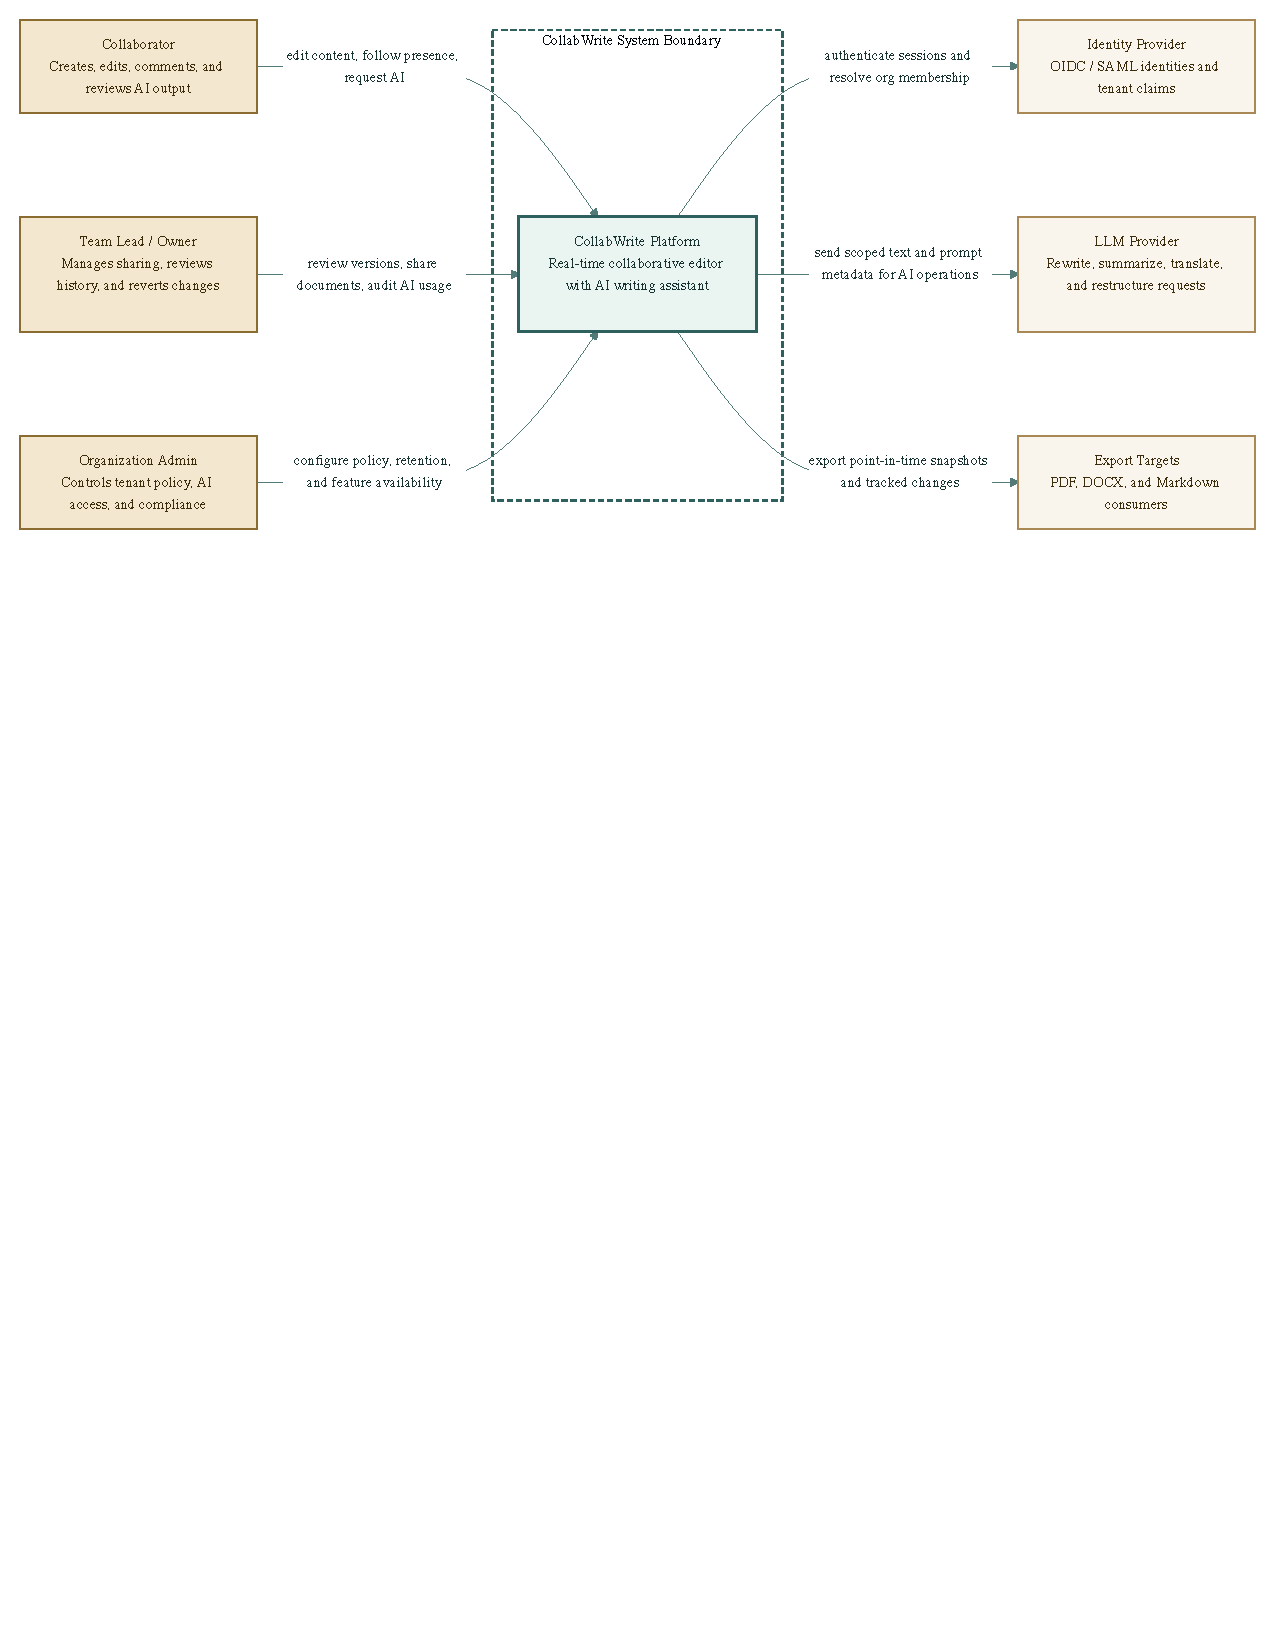
\includegraphics[width=\textwidth]{system-context.pdf}
    \caption{Level 1 system context diagram for \Repo{}.}
    \label{fig:system-context}
\end{figure}

The system context places \Repo{} between three human actor categories and three external systems. The most important external boundary is the LLM provider because it introduces privacy, latency, and cost trade-offs. Identity remains external as well so authentication can evolve without changing document-domain logic.

\subsubsection{Level 2: Container Diagram}

\begin{figure}[H]
    \centering
    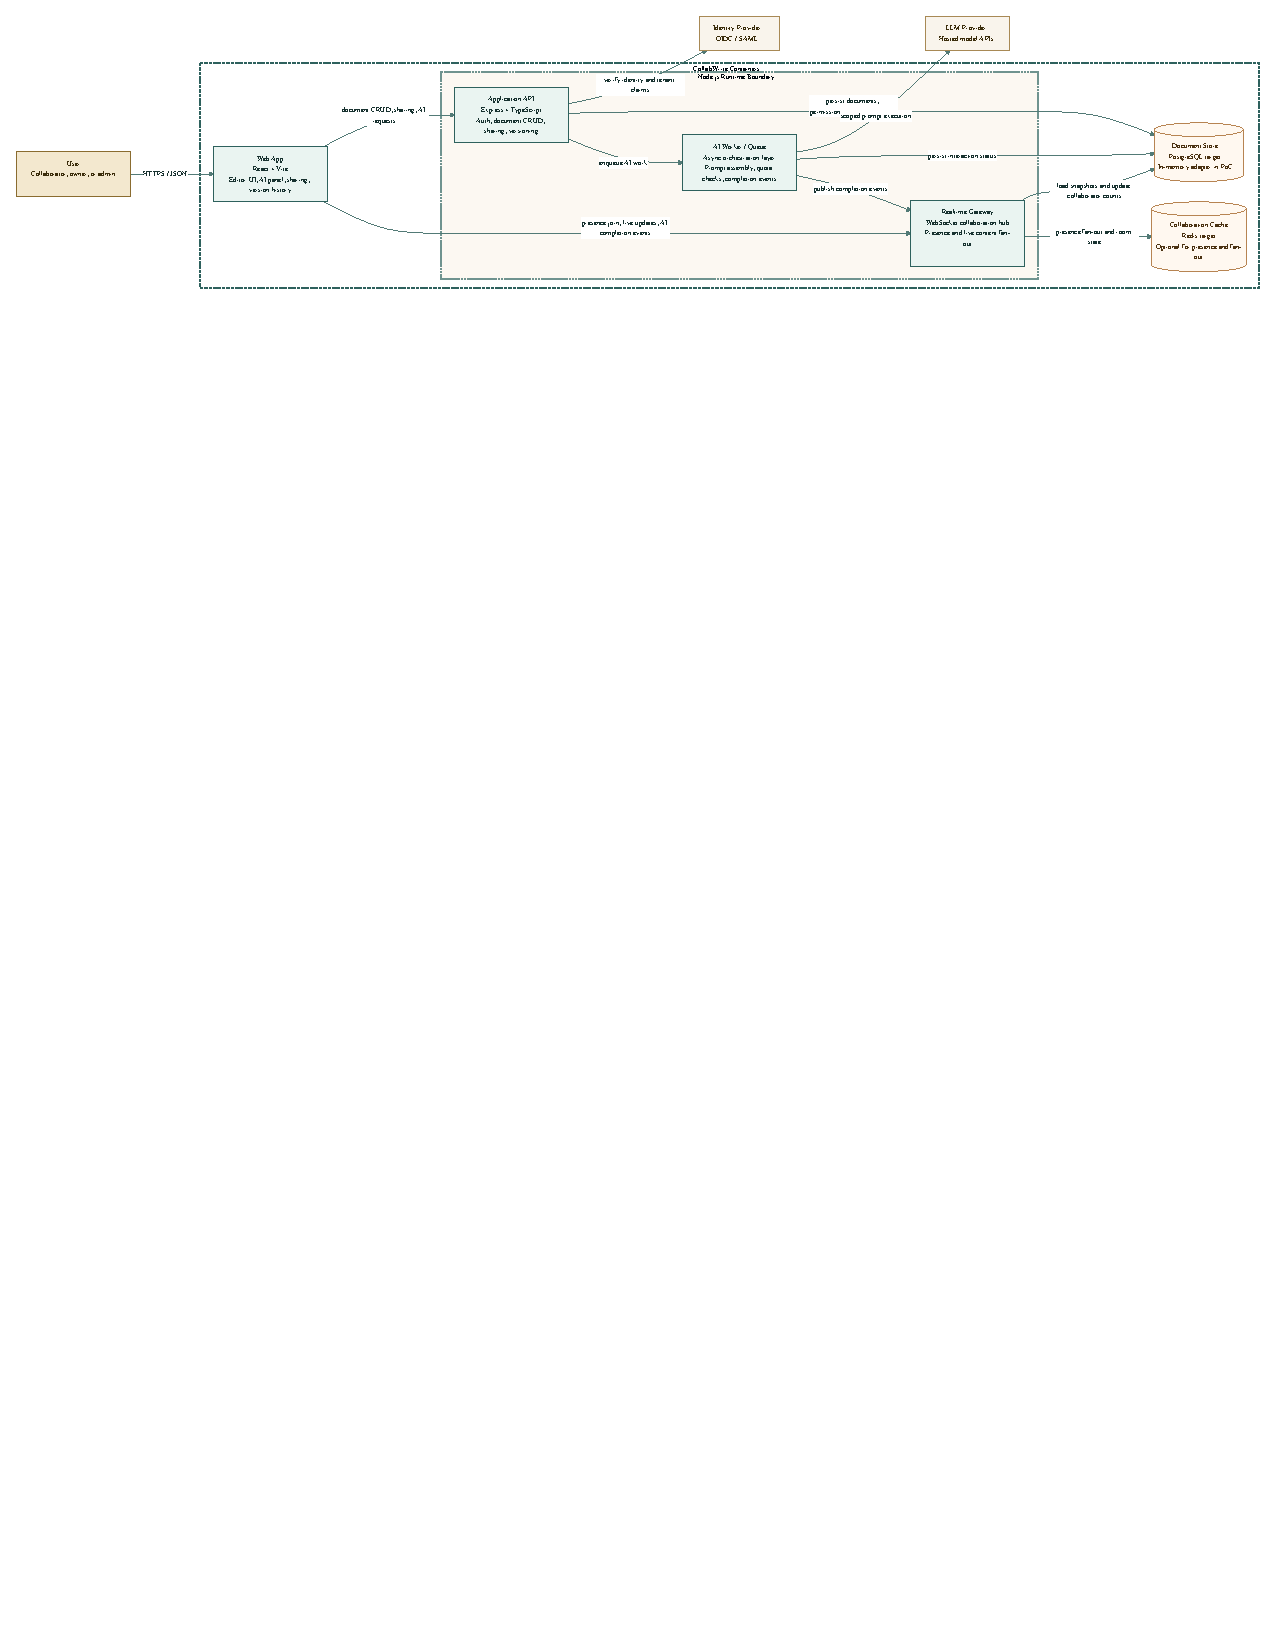
\includegraphics[width=\textwidth]{container.pdf}
    \caption{Level 2 container view for \Repo{}.}
    \label{fig:container}
\end{figure}

The container design separates the web client from the application API and the realtime collaboration gateway. In the PoC, the REST API and WebSocket gateway run in the same Node.js process, but they remain distinct containers logically because they solve different problems and will scale differently later. The implementation now also includes a dedicated FastAPI export worker so binary document rendering stays isolated from the interactive Node.js collaboration path. The target architecture also introduces an AI worker / queue boundary so long-running model calls do not block interactive API behavior.

\subsubsection{Level 3: Component Diagram for the Application API}

\begin{figure}[H]
    \centering
    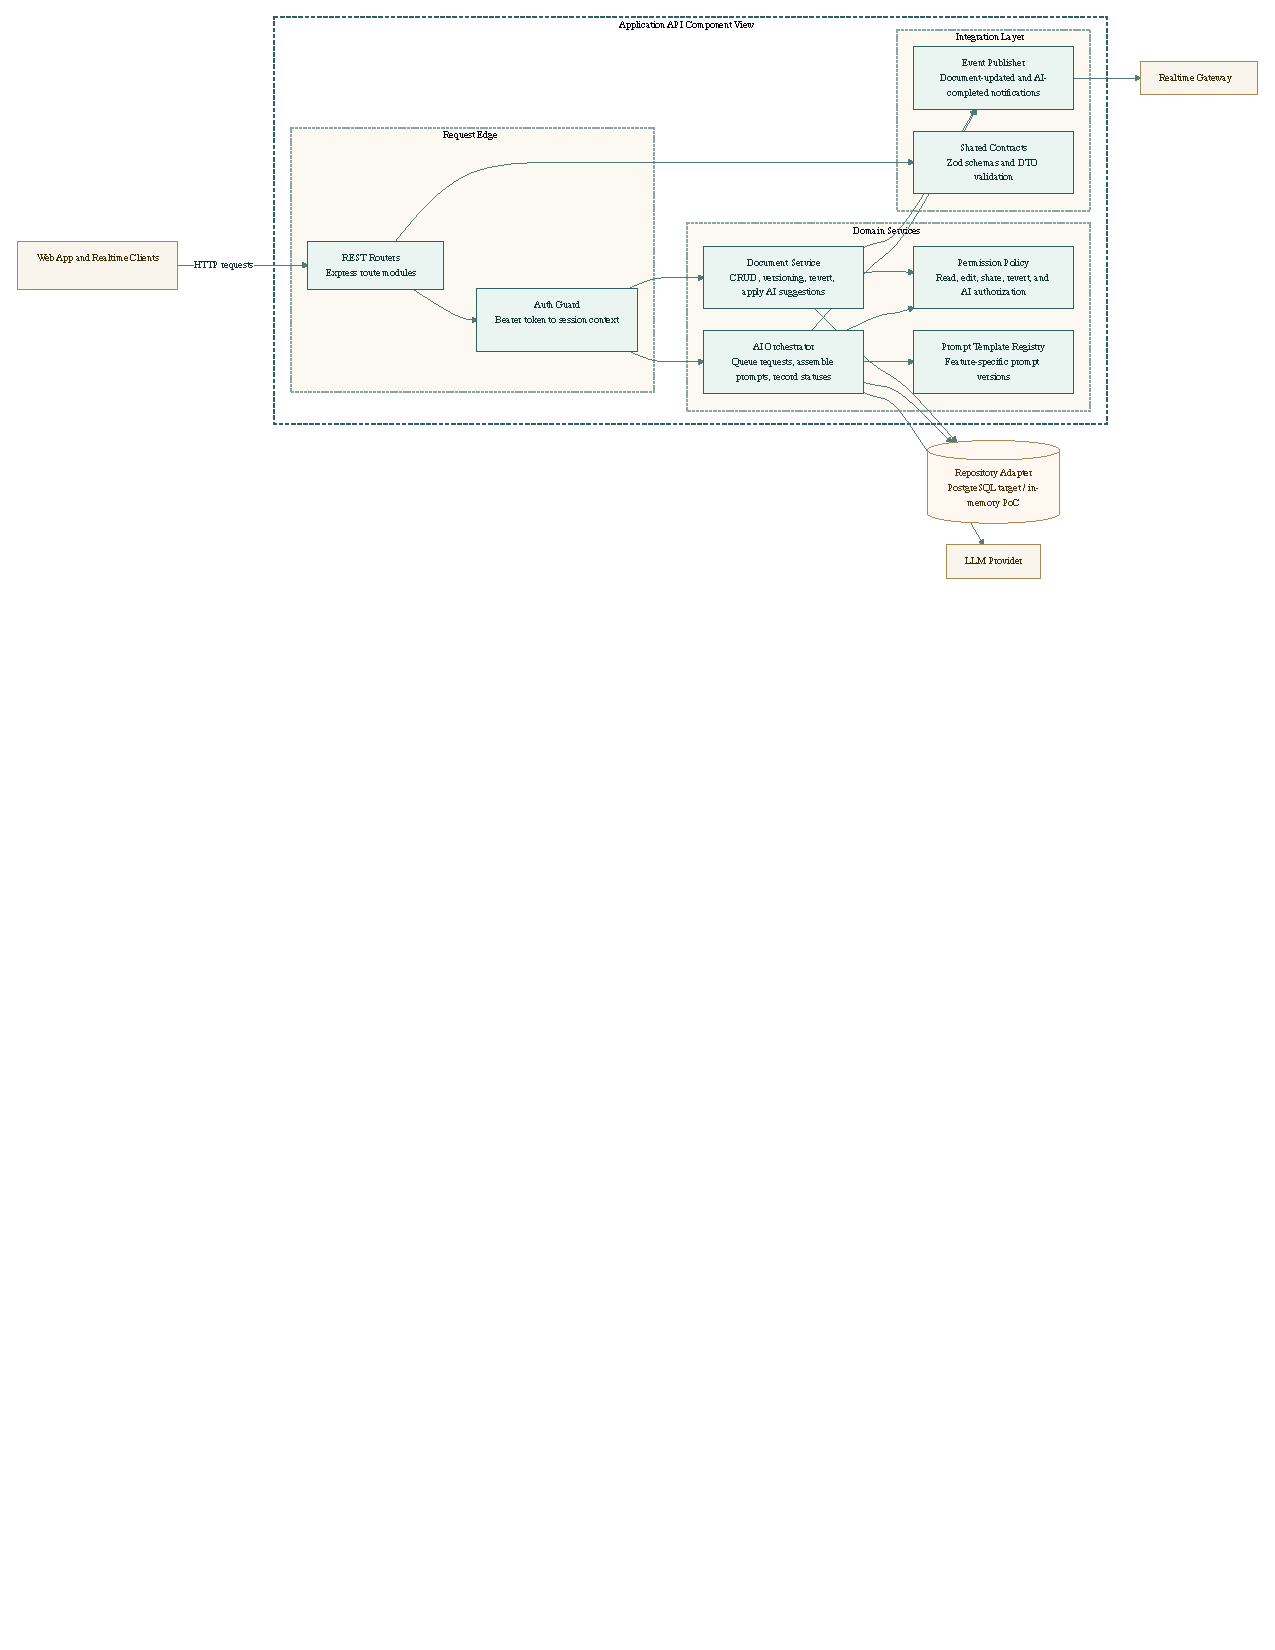
\includegraphics[width=\textwidth]{backend-components.pdf}
    \caption{Level 3 component view for the application API container.}
    \label{fig:backend-components}
\end{figure}

The application API container is the best Level 3 candidate because it contains most of the business rules: authorization, versioning, AI orchestration, and contract validation. The implemented PoC mirrors this decomposition through route modules, services, a collaboration hub, and an in-memory repository adapter.

Full Mermaid source listings for Figures~\ref{fig:system-context} to~\ref{fig:backend-components}, plus the data model and AI lifecycle diagrams, are provided in Appendix~\ref{app:mermaid}.

\subsubsection{Feature Decomposition}

\begin{longtblr}[
  caption = {Feature decomposition and module contracts},
  label = {tab:feature-decomposition}
]{
  width = \textwidth,
  colspec = {X[1.2,l] X[2.0,l] X[1.7,l] X[1.9,l]},
  rowhead = 1,
  row{1} = {bg=tableheader,fg=white,font=\bfseries},
  cells = {valign=t},
  hlines,
  vlines
}
Module & Responsibility & Depends on & Exposes \\
Web editor module & Owns text-editing UX, selection capture, document switching, and read-only behavior by role & Shared contracts, REST API, realtime gateway & Document view state, selection range, editor events \\
Frontend collaboration state & Tracks current document, current version, participants, reconnect state, and AI-panel state & WebSocket channel, shared message schemas & Presence UI, reconnect logic, socket message handlers \\
Realtime synchronization layer & Validates join context, tracks presence, applies live edits, and broadcasts updates & Auth service, document service, shared contracts & WebSocket session \texttt{/ws}, \texttt{presence.*}, \texttt{document.updated}, and \texttt{ai.completed} messages \\
AI assistant service & Persists AI interactions, scopes context, schedules async completion, enforces quota and policy, and selects the live or fallback provider & Document service, repository, OpenAI Responses adapter, or mock adapter & AI request creation, completion lifecycle, provider status, and suggestion updates \\
Document storage and versioning & Stores document aggregate, immutable versions, permissions, and AI history & Repository adapter & CRUD, version history, revert, share, and apply-suggestion operations \\
Export rendering service & Produces PDF, DOCX, and Markdown artifacts from point-in-time document snapshots and optional AI history & Application API, Python document libraries & \texttt{POST /render} and binary export payloads \\
Authentication and authorization & Resolves session tokens and enforces role rules plus \texttt{allowAi} & Session store, permission grants & Auth middleware, login endpoint, access decisions \\
Shared contract package & Maintains request/response/message schemas for web and API & Zod and TypeScript & \texttt{@midterm/shared} DTOs and runtime parsers \\
\end{longtblr}

\subsection{AI Integration Design}

\subsubsection{Context and Scope}

AI sees the explicit user selection by default, and the current implementation also passes a narrow surrounding context window for higher-quality rewrites plus a cursor-local context window for inline continuation. This minimizes privacy risk, reduces token cost, and improves prompt relevance without sending the full document body to the provider by default. For very long documents, the system still loads only the requested segment plus lightweight local context instead of the full draft.

\subsubsection{Trustworthiness of Cloud-Based Completion}

Inline completion is the most trust-sensitive AI feature in the PoC because it feels like local autocomplete while still depending on a cloud model. The design therefore uses a deliberately conservative contract:

\begin{enumerate}[leftmargin=1.4em]
    \item completion is explicit and user-triggered through the \texttt{Continue Writing} action rather than being sent on every keystroke;
    \item the provider receives only the document title plus bounded text immediately before and after the cursor, not the full draft by default;
    \item the UI exposes whether the system is using the live OpenAI provider or the fallback mock path;
    \item the returned text is treated as a proposal, not as silent ghost text, so the writer keeps editorial control;
    \item each interaction stores the initiator, model, prompt-template version, and requested document version for later inspection; and
    \item completion apply requests are rejected if the document changed in the meantime.
\end{enumerate}

This means the completion feature is cloud-based but still explainable in terms of bounded disclosure, explicit invocation, inspectable provenance, and safe application semantics. A production always-on autocomplete experience would require stronger tenant policy controls, retention guarantees, and provider evaluation before it should be trusted with high-sensitivity content.

\subsubsection{Suggestion UX}

AI output is presented as a tracked proposal in a side panel rather than as an immediate inline mutation. This design:

\begin{enumerate}[leftmargin=1.4em]
    \item keeps authors in control,
    \item makes AI history inspectable, and
    \item supports later partial-merge and tracked-change export workflows.
\end{enumerate}

The current PoC supports apply and reject. The target product also supports partial acceptance, which is already represented in the data model through the \texttt{partially\_applied} state.

\begin{figure}[H]
    \centering
    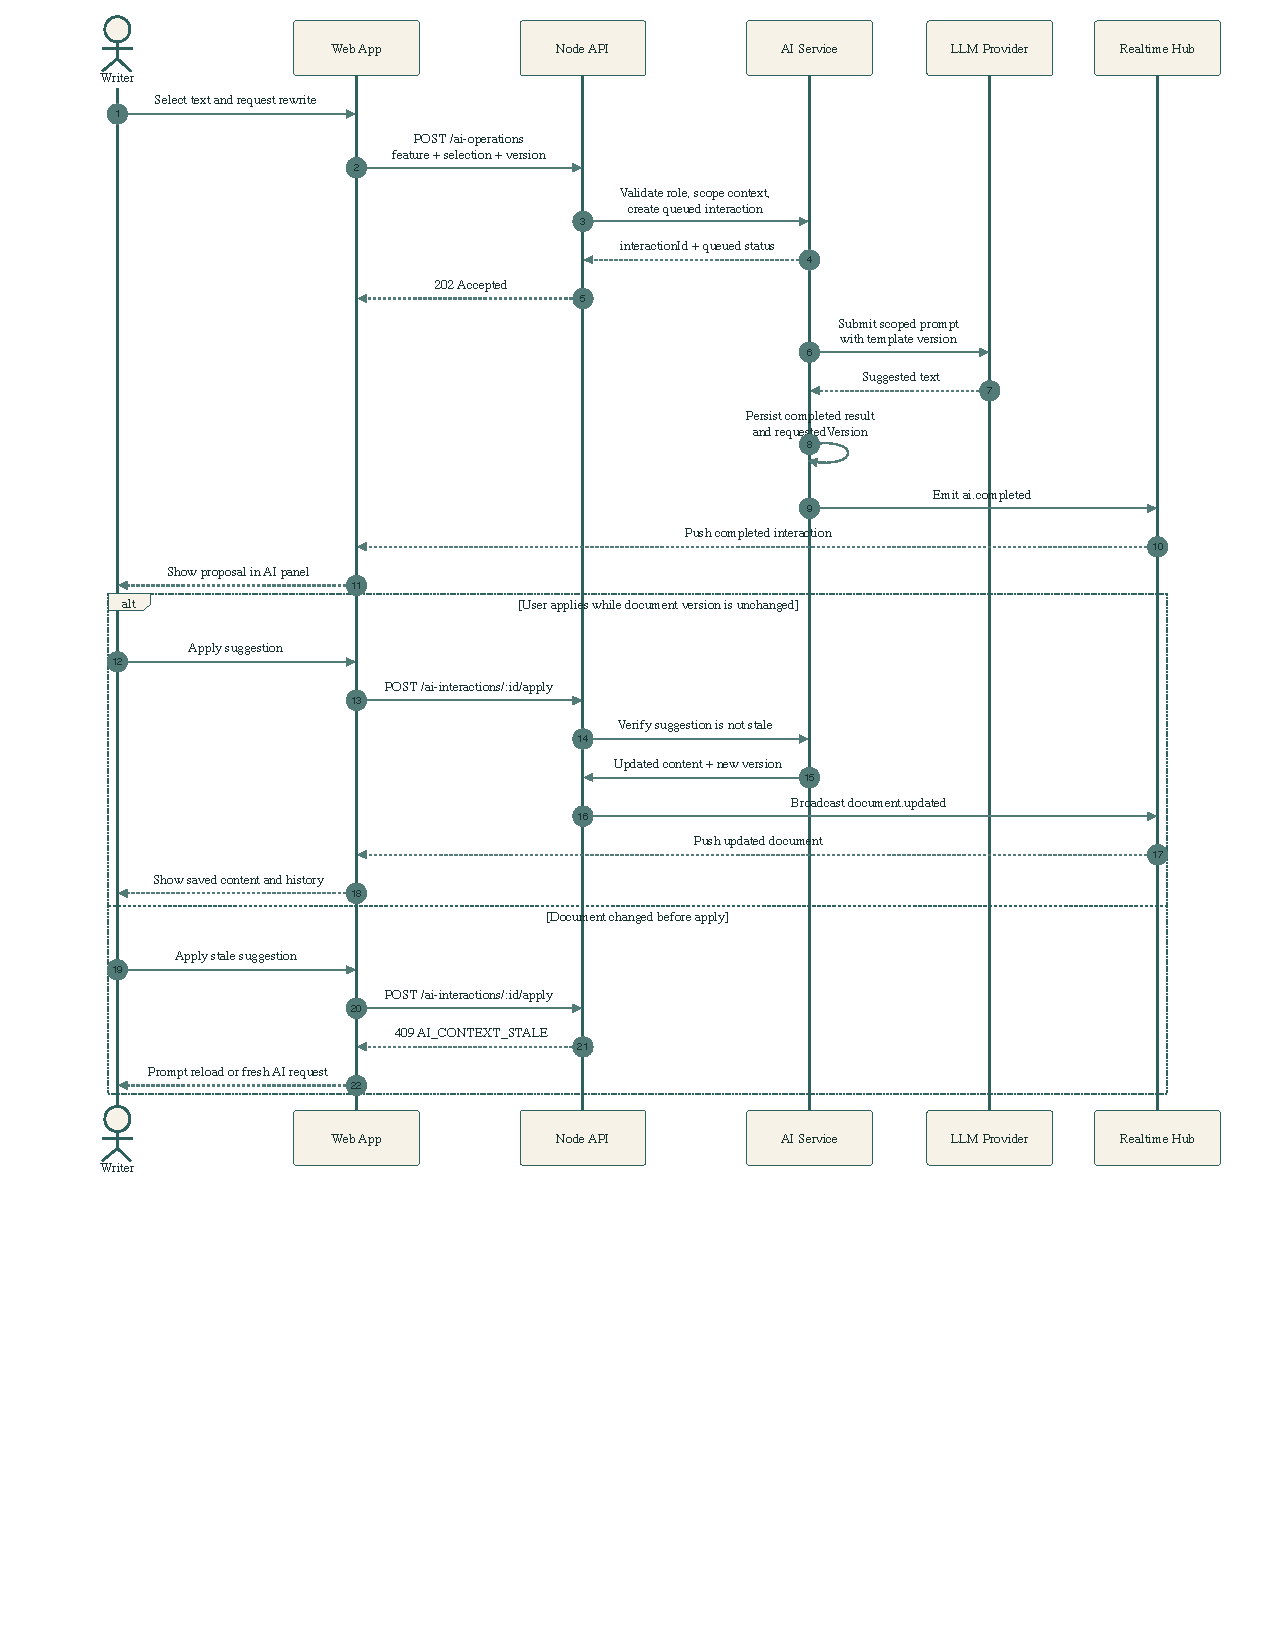
\includegraphics[width=\textwidth]{ai-lifecycle.pdf}
    \caption{Asynchronous AI suggestion lifecycle in the implemented PoC.}
    \label{fig:ai-lifecycle}
\end{figure}

Figure~\ref{fig:ai-lifecycle} makes one of the most important design choices explicit: AI is handled as an asynchronous proposal workflow rather than a synchronous content mutation. The client gets a fast acceptance response, the server performs prompt assembly and provider interaction out of band, and the final suggestion re-enters the user experience through the same realtime channel used for collaborative document updates.

\subsubsection{AI During Collaboration}

The system does not lock the selected region during AI generation. Other edits may continue. Because of that, completed suggestions are version-scoped: if the document changes after the request was created, the server rejects a blind apply attempt and forces the client to reload or request a fresh suggestion. If the user applies a still-valid suggestion, that application becomes a new version and is broadcast to the session like any other edit. This avoids pessimistic-locking complexity while preserving recoverability through version history.

\subsubsection{Prompt Design}

Prompt logic is template-based and versioned rather than hardcoded inside controllers. Each AI interaction records \texttt{promptTemplateVersion} so the team can compare behavior over time and revise prompts without losing traceability. The implemented provider layer also forces structured output parsing so the model returns only the insertion or replacement text expected by the editor.

\subsubsection{Model and Cost Strategy}

The implemented AI layer uses different model classes by task:

\begin{itemize}[leftmargin=1.3em]
    \item rewrite and restructure use a higher-quality model;
    \item summarize and translation use cheaper, faster models where acceptable;
    \item quota management combines per-user daily limits with tenant budget caps.
\end{itemize}

When quota is exceeded, the API returns a specific \texttt{quota\_exceeded} state so the client can distinguish this from a transient model failure. When the live provider is not configured, the same orchestration path falls back to a deterministic mock adapter so local development remains runnable.

\subsection{API Design}

\subsubsection{API Style}

The communication model deliberately mixes synchronous REST with asynchronous push:

\begin{itemize}[leftmargin=1.3em]
    \item REST handles CRUD, sharing, version history, login, and AI request creation because these actions are explicit, auditable, and easy to test.
    \item REST also brokers export requests because export is an explicit document-management operation that returns a point-in-time artifact.
    \item WebSocket handles presence and live content propagation because polling would degrade collaboration UX and waste resources.
\end{itemize}

\subsubsection{REST API Contract}

\begin{landscape}
\scriptsize
\begin{longtblr}[
  caption = {REST API contract},
  label = {tab:api-contract}
]{
  width = \linewidth,
  colspec = {X[1.2,l] X[1.5,l] X[1.8,l] X[1.8,l] X[1.7,l]},
  rowhead = 1,
  row{1} = {bg=tableheader,fg=white,font=\bfseries},
  cells = {valign=t},
  hlines,
  vlines
}
Interaction & Method and path & Request contract & Response contract & Notes \\
Login & \texttt{POST /v1/auth/login} & \texttt{\{ userId \}} & \texttt{\{ session, user \}} & PoC uses seeded users; production swaps to IdP-backed login \\
Session lookup & \texttt{GET /v1/auth/me} & Bearer token & \texttt{\{ session, user \}} & Validates token and refreshes client context \\
List users & \texttt{GET /v1/users} & none & \texttt{\{ users[] \}} & Used for demo login and sharing UI \\
AI provider status & \texttt{GET /v1/ai/provider} & Bearer token & \texttt{\{ provider \}} & Exposes whether the app is using live OpenAI or the fallback adapter \\
List documents & \texttt{GET /v1/documents} & Bearer token & \texttt{\{ documents[] \}} & Returns only documents visible to the caller \\
Create document & \texttt{POST /v1/documents} & \texttt{\{ title, content \}} & \texttt{\{ document \}} & Seeds initial owner permission and version 1 \\
Load document & \texttt{GET /v1/documents/:id} & Bearer token & \texttt{\{ document \}} & Returns content, permissions, versions, and AI history \\
Update content & \texttt{PUT /v1/documents/:id/content} & \texttt{\{ baseVersion, content, reason \}} & \texttt{\{ document, savedVersion \}} & Rejects stale base version \\
List versions & \texttt{GET /v1/documents/:id/versions} & Bearer token & \texttt{\{ versions[] \}} & Ordered newest-first \\
Revert version & \texttt{POST /v1/documents/:id/revert} & \texttt{\{ versionNumber \}} & \texttt{\{ document, savedVersion \}} & Creates a new top-of-history version \\
List permissions & \texttt{GET /v1/documents/:id/permissions} & Bearer token & \texttt{\{ permissions[] \}} & Used to inspect access state \\
Share document & \texttt{POST /v1/documents/:id/share} & \texttt{\{ principalType, principalId, role, allowAi \}} & \texttt{\{ permissions[] \}} & Owner-only operation \\
Export document & \texttt{POST /v1/documents/:id/export} & \texttt{\{ format, includeAiAppendix \}} & binary attachment & Proxies a snapshot to the FastAPI renderer and returns PDF, DOCX, or Markdown \\
List AI interactions & \texttt{GET /v1/documents/:id/ai-interactions} & Bearer token & \texttt{\{ interactions[] \}} & Supports reload and auditing \\
Request AI & \texttt{POST /v1/documents/:id/ai-operations} & \texttt{\{ feature, selection, targetLanguage? \}} & \texttt{\{ interaction \}} & Returns \texttt{202 Accepted} or \texttt{429} quota result \\
Apply AI suggestion & \texttt{POST /v1/documents/:id/ai-interactions/:iid/apply} & \texttt{\{ mode, acceptedText? \}} & \texttt{\{ document \}} & Creates a new version if content changes and rejects stale AI context \\
Reject AI suggestion & \texttt{POST /v1/documents/:id/ai-interactions/:iid/reject} & \texttt{\{\}} & \texttt{\{ interactions[] \}} & Marks the suggestion as rejected \\
\end{longtblr}
\normalsize
\end{landscape}

\subsubsection{Realtime Session Contract}

The client joins a document session through \url{ws://host/ws?token=<session>&documentId=<documentId>}. Server-to-client messages include \texttt{presence.snapshot}, \texttt{presence.updated}, \texttt{document.updated}, and \texttt{ai.completed}. Client-to-server messages include \texttt{document.change} and \texttt{cursor.change}.

\subsubsection{Long-Running AI Operations}

From the client perspective, AI is asynchronous:

\begin{enumerate}[leftmargin=1.4em]
    \item the client submits \texttt{POST /ai-operations};
    \item the API immediately returns a queued interaction record;
    \item the AI worker completes later and emits \texttt{ai.completed} over WebSocket;
    \item the client updates the side panel and waits for explicit apply or reject.
\end{enumerate}

This avoids long synchronous HTTP waits and distinguishes queue acceptance from model completion.

\subsubsection{Error Handling Strategy}

Clients distinguish failure modes by explicit error codes or interaction state:

\begin{itemize}[leftmargin=1.3em]
    \item AI slow: request accepted but interaction remains \texttt{queued} or \texttt{in\_progress};
    \item AI failed: interaction becomes \texttt{failed};
    \item quota exceeded: HTTP \texttt{429} with interaction state \texttt{quota\_exceeded};
    \item stale AI suggestion: HTTP \texttt{409} with \texttt{AI\_CONTEXT\_STALE};
    \item stale edit: HTTP or socket error \texttt{VERSION\_CONFLICT};
    \item unauthorized: \texttt{UNAUTHORIZED};
    \item forbidden action: \texttt{FORBIDDEN}, \texttt{EDIT\_NOT\_ALLOWED}, \texttt{SHARE\_NOT\_ALLOWED}, or \texttt{AI\_NOT\_ALLOWED}.
\end{itemize}

\subsection{Authentication and Authorization}

Authentication is required because the product manages private content and document-scoped permissions. The system expects regular collaborators, document owners or team leads, and organization administrators.

\begin{longtblr}[
  caption = {Document roles and permissions},
  label = {tab:roles}
]{
  width = \textwidth,
  colspec = {X[1.0,l] X[0.7,l] X[0.7,l] X[0.7,l] X[0.7,l] X[1.1,l]},
  rowhead = 1,
  row{1} = {bg=tableheader,fg=white,font=\bfseries},
  cells = {valign=t},
  hlines,
  vlines
}
Role & Read & Edit & Revert & Share & Invoke AI \\
Owner & Yes & Yes & Yes & Yes & Yes \\
Editor & Yes & Yes & Yes & No & If \texttt{allowAi=true} \\
Commenter & Yes & No & No & No & If \texttt{allowAi=true} \\
Viewer & Yes & No & No & No & No by default \\
\end{longtblr}

The most important privacy consideration is third-party AI processing. The design mitigates this by sending only scoped selections, logging prompt-template versions, and treating AI access as a separate policy knob rather than as a side effect of edit permission.

\subsection{Communication Model}

The communication model is hybrid and push-based:

\begin{itemize}[leftmargin=1.3em]
    \item initial open: the client authenticates, fetches the document bundle over REST, and then joins the WebSocket room;
    \item active editing: presence and edits propagate by push to keep latency low;
    \item connectivity loss: the client reconnects automatically and reloads the latest snapshot before resuming edits.
\end{itemize}

This model is more complex than polling, but it aligns with the top-ranked architectural driver: low-latency collaboration.

\subsection{Code Structure and Repository Organization}

\subsubsection{Monorepo vs.\ Multi-Repo}

The project uses a monorepo. With a small team and heavy shared-DTO usage, a monorepo is the lowest-friction option because it keeps web, API, and shared contracts versioned together. A multi-repo split would create unnecessary coordination cost every time request or response schemas evolve.

\subsubsection{Directory Layout}

\begin{lstlisting}[style=reportcode,caption={Repository layout},label={lst:repo-tree}]
.
|-- apps
|   |-- api
|   |   `-- src
|   |       |-- middleware
|   |       |-- realtime
|   |       |-- repositories
|   |       |-- routes
|   |       |-- services
|   |       |-- utils
|   |       |-- app.ts
|   |       |-- app.test.ts
|   |       `-- server.ts
|   `-- web
|       |-- index.html
|       `-- src
|           |-- components
|           |-- styles
|           |-- api.ts
|           |-- App.tsx
|           `-- main.tsx
|-- packages
|   `-- shared
|       `-- src
|           |-- index.ts
|           `-- index.test.ts
|-- services
|   `-- export-api
|       |-- main.py
|       |-- requirements.txt
|       `-- test_main.py
|-- docs
|   |-- diagrams
|   `-- report
|-- package.json
`-- README.md
\end{lstlisting}

\subsubsection{Shared Code}

Shared request, response, and realtime message schemas live in \texttt{packages/shared}. This package exposes Zod schemas plus inferred TypeScript types. The API uses them for runtime validation; the frontend uses them for compile-time safety and message handling.

\subsubsection{Configuration Management}

Secrets are environment-driven. The PoC needs variables such as \texttt{VITE\_API\_URL} and \texttt{EXPORT\_SERVICE\_URL}, while the production architecture expects LLM keys, database URLs, and session secrets to live in environment variables or a secret manager. \texttt{.env} files are ignored and \texttt{.env.example} documents the required keys.

\subsubsection{Testing Structure}

Tests sit next to source where practical:

\begin{itemize}[leftmargin=1.3em]
    \item \texttt{packages/shared/src/index.test.ts} for contract tests;
    \item \texttt{apps/api/src/app.test.ts} for API integration tests;
    \item \texttt{services/export-api/test\_main.py} for FastAPI export-worker tests.
\end{itemize}

Planned test layers include unit tests for prompt selection and permission policy, integration tests for REST contracts and repository behavior, and end-to-end tests for multi-user collaboration plus AI suggestion UX. AI integration is tested through deterministic provider stubs plus a mock-provider path so local and CI runs do not require paid API calls. Export integration is split cleanly: the Node.js API tests the proxy contract, while the Python worker tests binary rendering behavior directly.

\subsection{Data Model}

\begin{figure}[H]
    \centering
    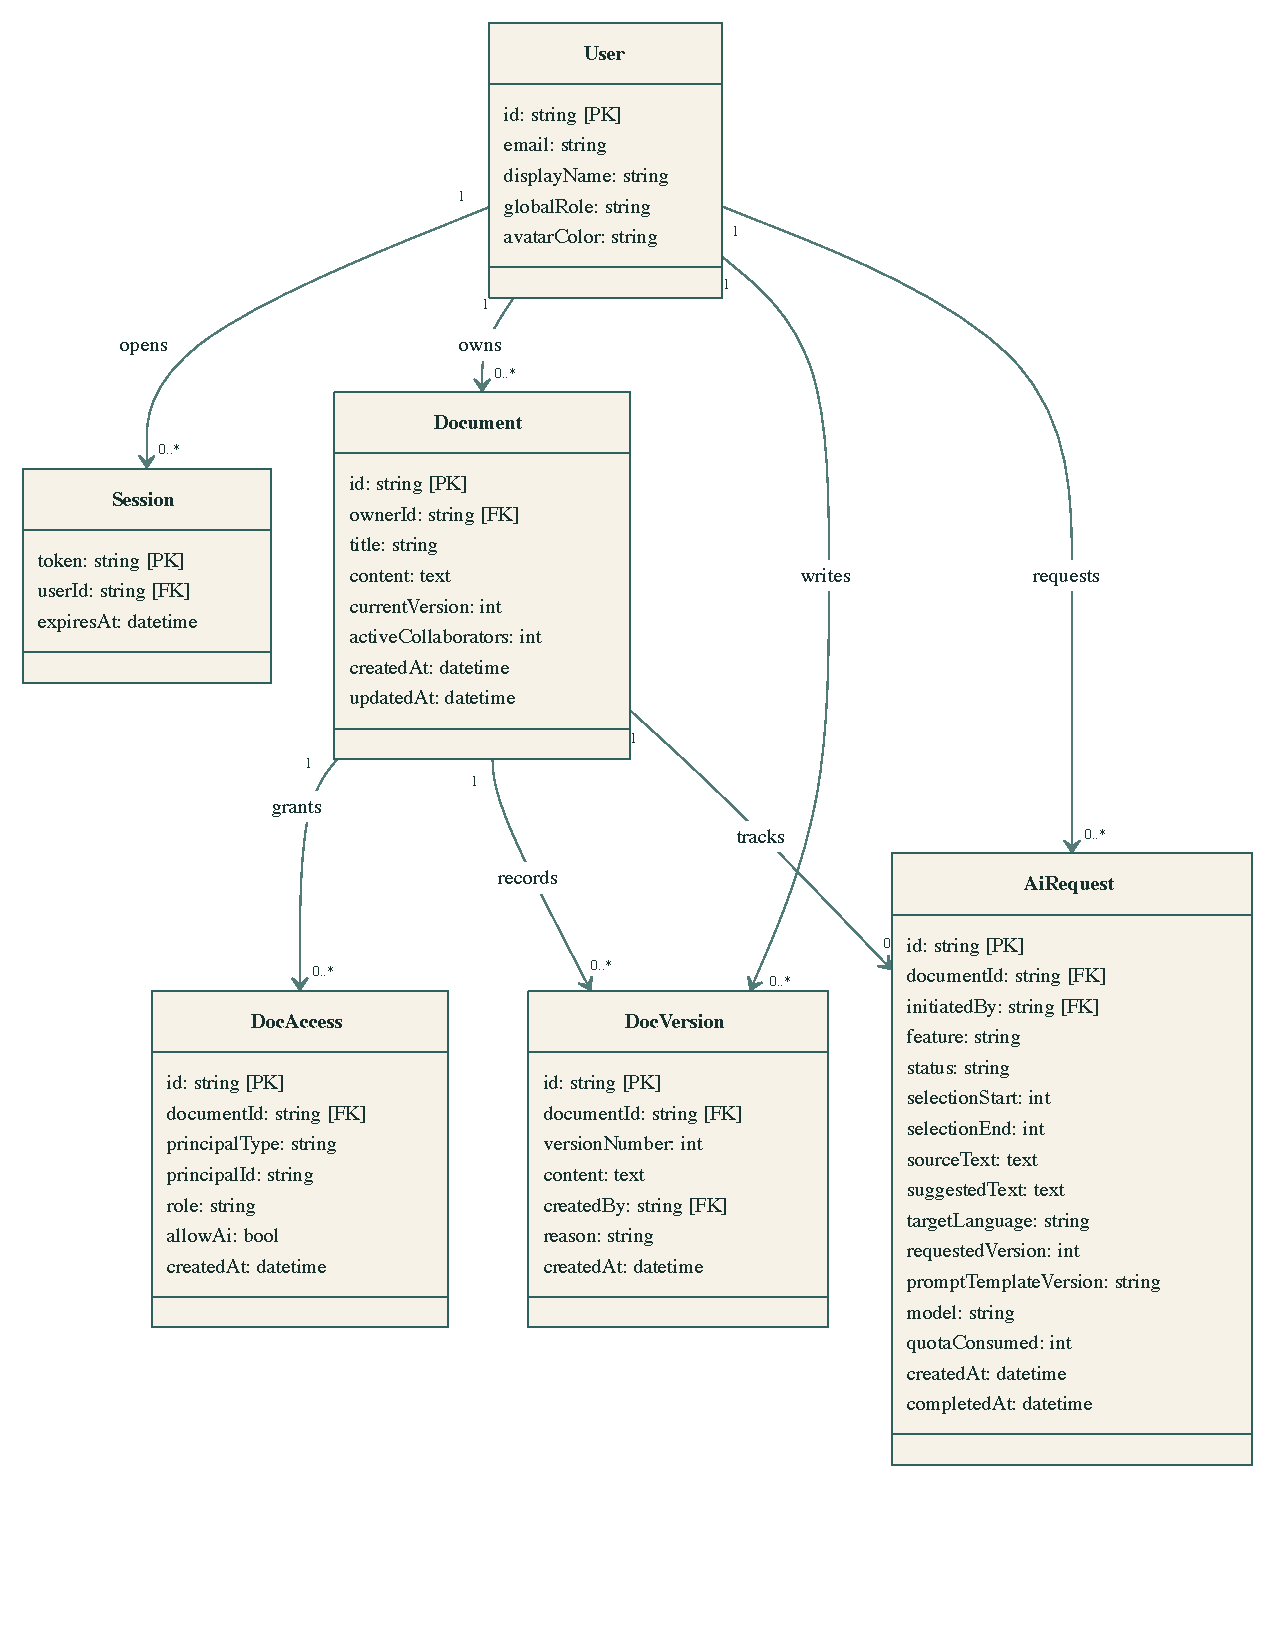
\includegraphics[width=\textwidth]{data-model.pdf}
    \caption{Logical data model diagram for the implemented PoC.}
    \label{fig:data-model}
\end{figure}

The document aggregate stores more than content: ownership, current version, timestamps, permissions, immutable versions, and AI interaction history. This is necessary because the product needs accountability, not just raw text storage. Three modeling decisions are especially consequential:

\begin{itemize}[leftmargin=1.3em]
    \item version history is immutable, so revert creates a new version rather than deleting old ones;
    \item AI interactions keep both source and suggested text so reviewers can compare and audit;
    \item permissions support users, teams, and link sharing even though the PoC currently implements user principals only.
\end{itemize}

\subsection{Architecture Decision Records}

\subsubsection{ADR-01: Monorepo with Shared Contract Package}

\begin{itemize}[leftmargin=1.3em]
    \item \textbf{Status:} Accepted
    \item \textbf{Context:} Web, API, and realtime flows evolve together. Schema drift would slow the team and break demos.
    \item \textbf{Decision:} Keep frontend, backend, and shared contracts in one repository and publish DTOs through an internal workspace package.
    \item \textbf{Consequences:} Faster cross-layer changes, easier traceability, and a single CI pipeline. The trade-off is a larger repository and less independent deployment freedom.
    \item \textbf{Alternatives considered:} Separate repos for web and backend were rejected because every API change would require cross-repo synchronization and duplicate type definitions.
\end{itemize}

\subsubsection{ADR-02: REST for CRUD plus WebSocket for Collaboration}

\begin{itemize}[leftmargin=1.3em]
    \item \textbf{Status:} Accepted
    \item \textbf{Context:} The system needs both strongly testable CRUD contracts and low-latency live editing.
    \item \textbf{Decision:} Use REST for explicit resource operations and WebSocket for presence plus content propagation.
    \item \textbf{Consequences:} Better UX and clearer boundaries, at the cost of maintaining two communication paths. That complexity is justified by the top-ranked latency driver.
    \item \textbf{Alternatives considered:} Polling was rejected because it increases latency and server load. An all-WebSocket design was rejected because it complicates auditable CRUD and testing.
\end{itemize}

\subsubsection{ADR-03: AI Suggestions Are Proposals, Not Immediate Mutations}

\begin{itemize}[leftmargin=1.3em]
    \item \textbf{Status:} Accepted
    \item \textbf{Context:} Direct AI mutation is fast to implement but reduces user trust and complicates collaboration recovery.
    \item \textbf{Decision:} AI writes suggestion records that users explicitly apply or reject.
    \item \textbf{Consequences:} Safer collaboration, easier auditing, and clearer version history. The trade-off is one extra interaction step for the user.
    \item \textbf{Alternatives considered:} Instant inline replacement was rejected because it hides AI provenance and increases accidental destructive edits.
\end{itemize}

\subsubsection{ADR-04: Repository Abstraction with In-Memory PoC Adapter}

\begin{itemize}[leftmargin=1.3em]
    \item \textbf{Status:} Accepted
    \item \textbf{Context:} The assignment requires a running PoC now, but the semester project will outgrow in-memory state quickly.
    \item \textbf{Decision:} Implement the PoC against an in-memory repository that already matches the future service and aggregate boundaries.
    \item \textbf{Consequences:} The demo remains lightweight while preserving a clean migration path to PostgreSQL and Redis later. The trade-off is that the PoC does not validate production persistence or multi-instance coordination yet.
    \item \textbf{Alternatives considered:} Hardwiring state directly inside route handlers was rejected because it would not scale architecturally or align with the report.
\end{itemize}

\clearpage
\section{Project Management and Team Collaboration}

\subsection{Team Structure and Ownership}

\begin{longtblr}[
  caption = {Team structure and ownership model},
  label = {tab:team-ownership}
]{
  width = \textwidth,
  colspec = {X[1.1,l] X[1.4,l] X[2.4,l]},
  rowhead = 1,
  row{1} = {bg=tableheader,fg=white,font=\bfseries},
  cells = {valign=t},
  hlines,
  vlines
}
Team member role & Ownership area & Responsibilities \\
Ahmed Aymna --- Backend / integration lead & \texttt{apps/api}, shared contracts, final integration & REST contracts, auth, sharing, versioning, export integration, cross-module merge resolution, and submission readiness \\
Aya --- Frontend / UX lead & \texttt{apps/web}, demo UX, interaction design & Editor UX, presence visualization, sharing and export affordances, AI-panel interaction flow, and demo polish \\
Mohamed Ibrahim --- Requirements / architecture lead & Requirements engineering, architecture narrative, report traceability & Stakeholder analysis, functional and non-functional requirements, user stories, traceability, and report consistency across sections \\
Praveen Anilkumar Shukla --- Realtime / AI / platform lead & \texttt{apps/api/realtime}, AI orchestration, environment setup & Realtime session behavior, observability, AI workflow coordination, provider integration boundaries, and runtime environment setup \\
\end{longtblr}

Features that span ownership, such as AI-assisted editing, are delivered through one cross-functional issue with explicit subtasks per owner and one designated integrator. Ahmed Aymna acts as the final integrator for submission branches, while Mohamed Ibrahim owns consistency between implemented behavior and the written report. Technical disagreements follow a lightweight ADR or RFC process; unresolved issues escalate to Ahmed Aymna plus one additional cross-area reviewer within 24 hours.

\subsection{Development Workflow}

\begin{itemize}[leftmargin=1.3em]
    \item \textbf{Branching strategy:} short-lived feature branches from \texttt{main}, named \texttt{feat/<scope>-<ticket>}, \texttt{fix/<scope>-<ticket>}, or \texttt{docs/<scope>-<ticket>}.
    \item \textbf{Merge policy:} pull requests only; no direct pushes to \texttt{main}; squash merge after review.
    \item \textbf{Code review:} at least one approving review from the owning area and one cross-area reviewer for shared contracts or cross-cutting features.
    \item \textbf{Approval criteria:} passing tests, no schema drift, updated docs for new endpoints, and clear rollback behavior for risky changes.
    \item \textbf{Issue tracking:} backlog items in GitHub Projects or Jira with labels such as \texttt{web}, \texttt{api}, \texttt{ai}, \texttt{realtime}, and \texttt{infra}.
    \item \textbf{Communication:} Slack or Microsoft Teams for daily coordination; durable decisions are copied into ADRs or issue comments so they do not disappear in chat history.
\end{itemize}

\subsection{Development Methodology}

The team uses a lightweight Scrum-style methodology with one-week iterations from \textbf{April 5, 2026} through \textbf{May 24, 2026}. Work is prioritized by architectural dependency first and user-visible value second:

\begin{enumerate}[leftmargin=1.4em]
    \item shared contracts and repository boundaries,
    \item document CRUD and auth,
    \item realtime editing and presence,
    \item AI workflow and quota handling,
    \item export and hardening.
\end{enumerate}

Infrastructure, testing, and data-model work are tracked as first-class backlog items with acceptance criteria, not treated as side work.

\subsection{Risk Assessment}

\footnotesize
\begin{longtblr}[
  caption = {Project-specific risk register},
  label = {tab:risk-register}
]{
  width = \textwidth,
  colspec = {X[1.5,l] X[0.8,l] X[1.4,l] X[1.8,l] X[1.8,l]},
  rowhead = 1,
  row{1} = {bg=tableheader,fg=white,font=\bfseries},
  cells = {valign=t},
  hlines,
  vlines
}
Risk & Likelihood & Impact & Mitigation & Contingency \\
Real-time edit conflicts become too frequent with naive full-document updates & Medium & Users lose trust in collaboration and edits may be overwritten & Move from full-document pushes to OT/CRDT or patch-based operations; add conflict telemetry early & Freeze simultaneous same-region editing and fall back to optimistic locking plus explicit conflict-resolution UI \\
Third-party AI latency or outages degrade the whole product & High & AI feels broken, but editing must continue & Keep AI asynchronous, decouple through a queue, and surface retryable states & Disable AI features temporarily while preserving editing, sharing, and history \\
AI cost grows unpredictably with large selections and repeated requests & Medium & Budget overrun or forced throttling & Enforce scoped context, quotas, tenant budget caps, and prompt templates by feature & Reduce available AI features or switch to lower-cost models for non-critical tasks \\
Schema drift between frontend and backend breaks integration late in the sprint & Medium & Demo failures and lost integration time & Keep shared contracts in a workspace package and test responses against schemas & Temporarily freeze feature work and repair contract mismatches before resuming \\
Ownership boundaries fail and cross-cutting features merge poorly & Medium & Integration stalls, PRs become large, and bug rates increase & Use clear module ownership, small PRs, and an explicit integrator for cross-functional work & Re-scope the sprint, assign one engineer to integration-only work, and defer lower-priority features \\
\end{longtblr}
\normalsize

\subsection{Timeline and Milestones}

\begin{longtblr}[
  caption = {Semester timeline and milestones},
  label = {tab:timeline}
]{
  width = \textwidth,
  colspec = {X[0.8,l] X[1.4,l] X[2.8,l]},
  rowhead = 1,
  row{1} = {bg=tableheader,fg=white,font=\bfseries},
  cells = {valign=t},
  hlines,
  vlines
}
Date & Milestone & Acceptance criteria \\
April 7, 2026 & Contract baseline complete & Shared DTO package exists; login and document CRUD schemas are agreed and reviewed. \\
April 14, 2026 & Authenticated CRUD slice complete & API serves document create/load/update with auth; integration tests pass. \\
April 21, 2026 & Realtime collaboration slice complete & Two clients can join the same document, see presence, and receive shared edits under target demo conditions. \\
April 28, 2026 & Versioning and sharing complete & Version history and owner-managed permission updates work through the UI and API. \\
May 8, 2026 & AI proposal workflow complete & AI requests queue asynchronously, suggestions appear in the UI, and apply/reject flows persist status correctly. \\
May 17, 2026 & Hardening sprint complete & README, diagrams, ADRs, risk register, tests, and environment setup are current; demo script is rehearsed. \\
May 24, 2026 & Final submission candidate & End-to-end demo passes from a fresh clone, the report is exported to PDF, and repository state is submission-ready. \\
\end{longtblr}

\clearpage
\section{Proof of Concept}

\subsection{What the PoC Demonstrates}

The implemented PoC validates the architectural skeleton directly in code:

\begin{itemize}[leftmargin=1.3em]
    \item a working React frontend in \texttt{apps/web};
    \item a working Express API in \texttt{apps/api};
    \item shared Zod contracts in \texttt{packages/shared};
    \item a dedicated FastAPI export worker in \texttt{services/export-api};
    \item authenticated document listing and loading;
    \item document creation, sharing, version history, and revert;
    \item role-aware AI request, proposal, apply, and reject flow;
    \item live OpenAI-backed rewrite, summarize, translate, restructure, proofread, and inline-completion workflows with a mock fallback path;
    \item export of point-in-time document snapshots to PDF, DOCX, and Markdown with an optional AI-history appendix;
    \item WebSocket presence and live content propagation.
\end{itemize}

\subsection{What the PoC Intentionally Does Not Implement Yet}

\begin{itemize}[leftmargin=1.3em]
    \item production identity-provider integration;
    \item persistent PostgreSQL or Redis infrastructure;
    \item OT/CRDT-grade merge logic for same-character concurrent edits;
    \item tenant billing, provider-routing policy, and enterprise governance controls around AI usage.
\end{itemize}

These omissions are deliberate. The PoC proves the contracts, module boundaries, and communication model without pretending the prototype is already production-ready.

\subsection{Architecture-to-Code Alignment}

\begin{longtblr}[
  caption = {Architecture-to-code alignment},
  label = {tab:architecture-alignment}
]{
  width = \textwidth,
  colspec = {X[1.4,l] X[2.6,l]},
  rowhead = 1,
  row{1} = {bg=tableheader,fg=white,font=\bfseries},
  cells = {valign=t},
  hlines,
  vlines
}
Architecture element & PoC implementation \\
Web app container & \texttt{apps/web} React client \\
Application API container & \texttt{apps/api} Express app and route modules \\
Realtime gateway & \texttt{apps/api/src/realtime/collaboration-hub.ts} \\
Export rendering worker & \texttt{services/export-api/main.py} FastAPI service for PDF, DOCX, and Markdown \\
Shared contracts & \texttt{packages/shared/src/index.ts} \\
Document store & \texttt{apps/api/src/repositories/in-memory-store.ts} as the PoC adapter \\
AI orchestrator & \texttt{apps/api/src/services/ai-service.ts} with async suggestion completion \\
\end{longtblr}

\subsection{How to Run the PoC}

Use the root-level commands:

\begin{lstlisting}[style=reportcode,caption={PoC setup and run commands},label={lst:poc-run}]
npm install
python3 -m venv .venv-export
source .venv-export/bin/activate
python3 -m pip install -r services/export-api/requirements.txt
npm run dev
npm run dev:export
\end{lstlisting}

Frontend: \url{http://localhost:5173} \\
Backend: \url{http://localhost:4000} \\
Export worker: \url{http://127.0.0.1:8000}

\subsection{Verification Evidence}

The repository passes the following verification commands:

\begin{itemize}[leftmargin=1.3em]
    \item \texttt{npm run typecheck}
    \item \texttt{npm test}
    \item \texttt{source .venv-export/bin/activate \&\& npm run test:export}
    \item \texttt{npm run build}
    \item \texttt{npm run render:report}
\end{itemize}

The backend was also smoke-tested through live \texttt{curl} requests against \texttt{/health}, \texttt{POST /v1/auth/login}, \texttt{GET /v1/documents}, the authenticated AI-provider status route, and the FastAPI export-renderer health endpoint. The PoC therefore demonstrates a working end-to-end slice rather than a disconnected UI mockup.

\clearpage

\appendix
\section{Mermaid Source Listings}\label{app:mermaid}

This appendix contains the Mermaid source for each rendered architecture diagram included in the main report. The sources remain editable and versionable in the repository.

\subsection{System Context Diagram}
\lstinputlisting[
  style=reportcode,
  caption={Mermaid source for the system context diagram},
  label={lst:system-context-mermaid}
]{../diagrams/system-context.mmd}

\subsection{Container Diagram}
\lstinputlisting[
  style=reportcode,
  caption={Mermaid source for the container diagram},
  label={lst:container-mermaid}
]{../diagrams/container.mmd}

\subsection{Backend Component Diagram}
\lstinputlisting[
  style=reportcode,
  caption={Mermaid source for the backend component diagram},
  label={lst:backend-components-mermaid}
]{../diagrams/backend-components.mmd}

\subsection{Data Model Diagram}
\lstinputlisting[
  style=reportcode,
  caption={Mermaid source for the data model diagram},
  label={lst:data-model-mermaid}
]{../diagrams/data-model.mmd}


\end{document}
